%\title{LaTeX Portrait Poster Template}
%%%%%%%%%%%%%%%%%%%%%%%%%%%%%%%%%%%%%%%%%
% a0poster Portrait Poster
% LaTeX Template
% Version 1.0 (22/06/13)
%
% The a0poster class was created by:
% Gerlinde Kettl and Matthias Weiser (tex@kettl.de)
% 
% Adapter by Jens Buysse for Hogeschool Gent
% This template has been downloaded from:
% http://www.LaTeXTemplates.com
%
% License:
% CC BY-NC-SA 3.0 (http://creativecommons.org/licenses/by-nc-sa/3.0/)
%
%%%%%%%%%%%%%%%%%%%%%%%%%%%%%%%%%%%%%%%%%

%----------------------------------------------------------------------------------------
%	PACKAGES AND OTHER DOCUMENT CONFIGURATIONS
%----------------------------------------------------------------------------------------

\documentclass[a0,portrait]{a0poster}

\usepackage{multicol} % This is so we can have multiple columns of text side-by-side
\columnsep=100pt % This is the amount of white space between the columns in the poster
\columnseprule=3pt % This is the thickness of the black line between the columns in the poster

\usepackage[svgnames]{xcolor} % Specify colors by their 'svgnames', for a full list of all colors available see here: http://www.latextemplates.com/svgnames-colors

\usepackage{times} % Use the times font
%\usepackage{palatino} % Uncomment to use the Palatino font

\usepackage{graphicx} % Required for including images
\graphicspath{{figures/}} % Location of the graphics files
\usepackage{booktabs} % Top and bottom rules for table
\usepackage[font=small,labelfont=bf]{caption} % Required for specifying captions to tables and figures
\usepackage{amsfonts, amsmath, amsthm, amssymb} % For math fonts, symbols and environments
\usepackage{wrapfig} % Allows wrapping text around tables and figures
\usepackage[export]{adjustbox}

\begin{document}

%----------------------------------------------------------------------------------------
%	POSTER HEADER 
%----------------------------------------------------------------------------------------

% The header is divided into two boxes:
% The first is 75% wide and houses the title, subtitle, names, university/organization and contact information
% The second is 25% wide and houses a logo for your university/organization or a photo of you
% The widths of these boxes can be easily edited to accommodate your content as you see fit

\begin{minipage}[t]{0.75\linewidth}
\VeryHuge \color{HoGentAccent1} \textbf{Docker of alternatieven als introductie tot container virtualisatie} \color{Black}\\ % Title
%%\Huge\textit{Ondertitel (eventueel)}\\[2.4cm] % Subtitle
\huge \textbf{Arents Eckhart, Van Vreckem Bert}\\[0.5cm] % Author(s)
\huge Hogeschool Gent, Valentin Vaerwyckweg 1, 9000 Gent\\[0.4cm] % University/organization
\Large \texttt{Eckhart.Arents@hogent.be} \\
\end{minipage}
%
\begin{minipage}[t]{0.25\linewidth}

\includegraphics[width=13cm,right]{figures/HOGENT_Logo_Pos_rgb.png} 

\end{minipage}

\vspace{1cm} % A bit of extra whitespace between the header and poster content

%----------------------------------------------------------------------------------------

\begin{multicols}{2} % This is how many columns your poster will be broken into, a portrait poster is generally split into 2 columns

%----------------------------------------------------------------------------------------
%	ABSTRACT
%----------------------------------------------------------------------------------------

\color{HoGentAccent1} % Navy color for the abstract

\begin{abstract}
Een onderzoek naar software voor container virtualisatie en verwante technologieën die kan gebruikt worden als leermiddel voor een student. Hiertoe werd eerst een onderzoek naar alle aanbieders van technologieën uitgevoerd, om ze vervolgens uit te proberen en in te schatten welke de meest geschikte is. Zo werden Docker en Podman beide beoordeeld als meest geschikte container engines en Kubernetes als beste leermiddel voor orchestration.
\end{abstract}
%----------------------------------------------------------------------------------------
%	INTRODUCTION
%----------------------------------------------------------------------------------------

\color{HoGentAccent1} 
\section*{Introductie}
\color{black}
\color{black}
Container virtualisatie is een alternatieve manier om te virtualiseren ten opzichte van de klassieke virtuele machine. Bij container virtualisatie wordt een applicatie die uitgevoerd word enkel voorzien van wat het nodig heeft. Hierdoor zijn containers lichter in gebruik dan virtuele machines en ook populair in cloud omgevingen. De technologie voor container virtualisatie is recent populair geworden dankzij Docker, maar komt echter nog niet aan bod binnen de opleiding toegepaste informatica aan de HoGent. In dit onderzoek werden Docker en alternatieven onderzocht naar hun geschiktheid om de volledige levenscyclus van een container beter te leren begrijpen.

Hiervoor werd eerst gekeken naar de mogelijkheden voor het effectief draaien van containers, de engine, en bijhorende container types. Verder werden alle software aanbiedingen voor het beheren van meerdere containers, zogenaamde orchestration software, afgetoetst. Ook werd gezocht naar mogelijke alternatieven voor de Docker hub voor het delen van containers. Ten slotte werden de container virtualisatie mogelijkheden van de grote cloud hosting services bekeken.
%----------------------------------------------------------------------------------------
%	GEOLOGY
%----------------------------------------------------------------------------------------

\color{Black} % DarkSlateGray color for the rest of the content
\color{HoGentAccent1} 
\section*{Experimenten}
\color{black}
Er werd praktijkgericht te werk gegaan door te vertrekken van de meest toegankelijke software voor de engines en de orchestration. Zo werd onderzocht hoe de Docker engine werkt op Windows als deel van de Docker desktop applicatie. Dit werd vergeleken met Podman in een Fedora virtuele machine. Ook werd Podman getest in een andere Linux omgeving met een Ubuntu virtuele machine.

Voor orchestration werd onderzocht hoe Kubernetes werkt als onderdeel van de Docker desktop applicatie. Dit werd dan vergeleken met Kubernetes die met Podman werkt en HashiCorp Nomad als orchestration software.

Ten slotte is er tussendoor ook onderzocht hoe het werken met de Docker Hub of de GitHub Container Registry van elkaar verschillen of niet qua gebruik, zowel in Docker als in Podman.

\color{HoGentAccent1} 
\section*{Sectie met figuur}
\color{black}


\begin{center}\vspace{1cm}
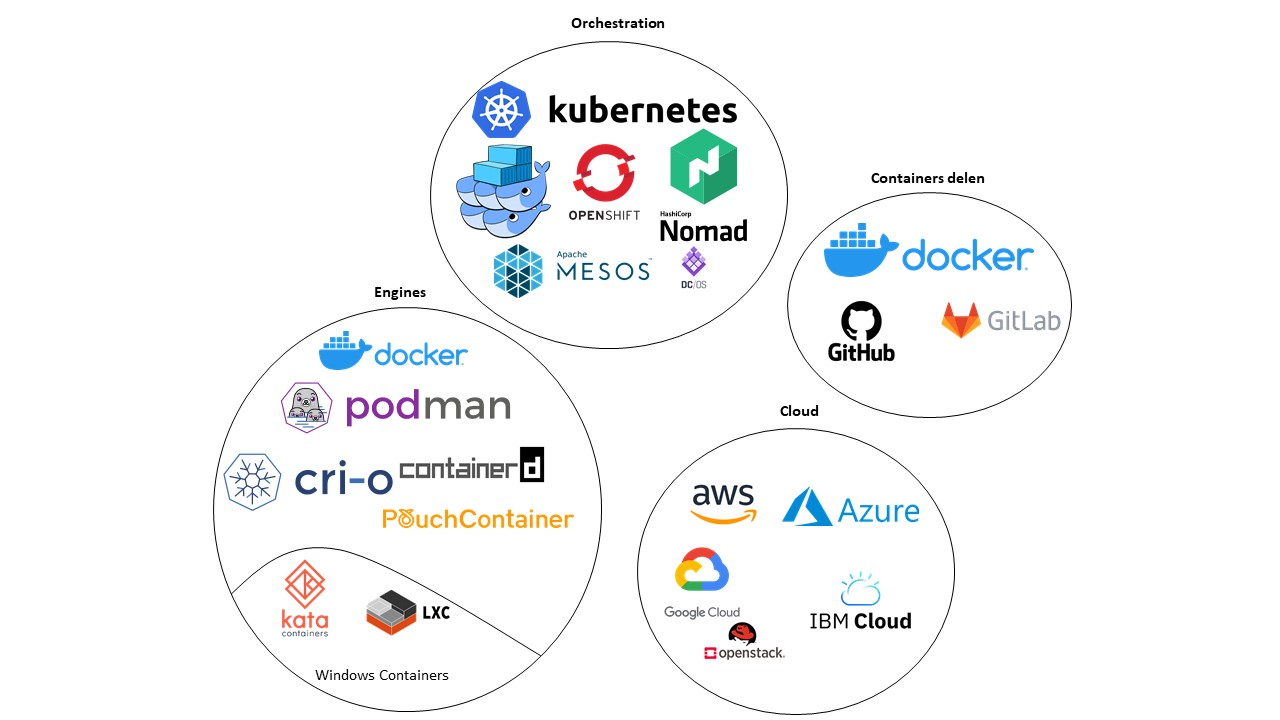
\includegraphics[width=1.0\linewidth]{software}
\captionof{figure}{\color{HoGentAccent5}De Gevonden software en service aanbieders gebundeld per categorie}
\end{center}\vspace{1cm}

%------------------------------------------------



\color{HoGentAccent1} 
\section*{Conclusies}
\color{black}
In het algemeen kan gesteld worden dat veel van de technologieën nood hebben aan Linux als onderliggend besturingssysteem en dat voor velen een virtuele machine nodig zal zijn. Tussen Docker en Podman is er weinig verschil te vinden. Podman is mogelijk iets complexer dan Docker door de ingebouwde “pods”. Voor orchestration is Kubernetes duidelijk de beste dankzij een uitstekende dashboard interface en ruimere ondersteuning dan Nomad. Voor het delen van containers wordt de Docker Hub het meest gebruikt. De GitHub Container Registry is een goed alternatief maar nog in bèta.
%----------------------------------------------------------------------------------------
%	FORTHCOMING RESEARCH
%----------------------------------------------------------------------------------------
\color{HoGentAccent1} 
\section*{Toekomstig onderzoek}
\color{black}

De mate waarin de GitHub Container Registry beter is dan de Docker Hub voor een gebruiker zou moeten worden heronderzocht worden eens de bèta hiervan afgelopen is. Ook is er ruimte om te onderzoeken hoe geschikt de cloud hosting services kunnen zijn om een student toe te laten om met cloud en containers gecombineerd te leren werken.


%----------------------------------------------------------------------------------------

\end{multicols}
\end{document}